\chapter{Natural Language Processing}

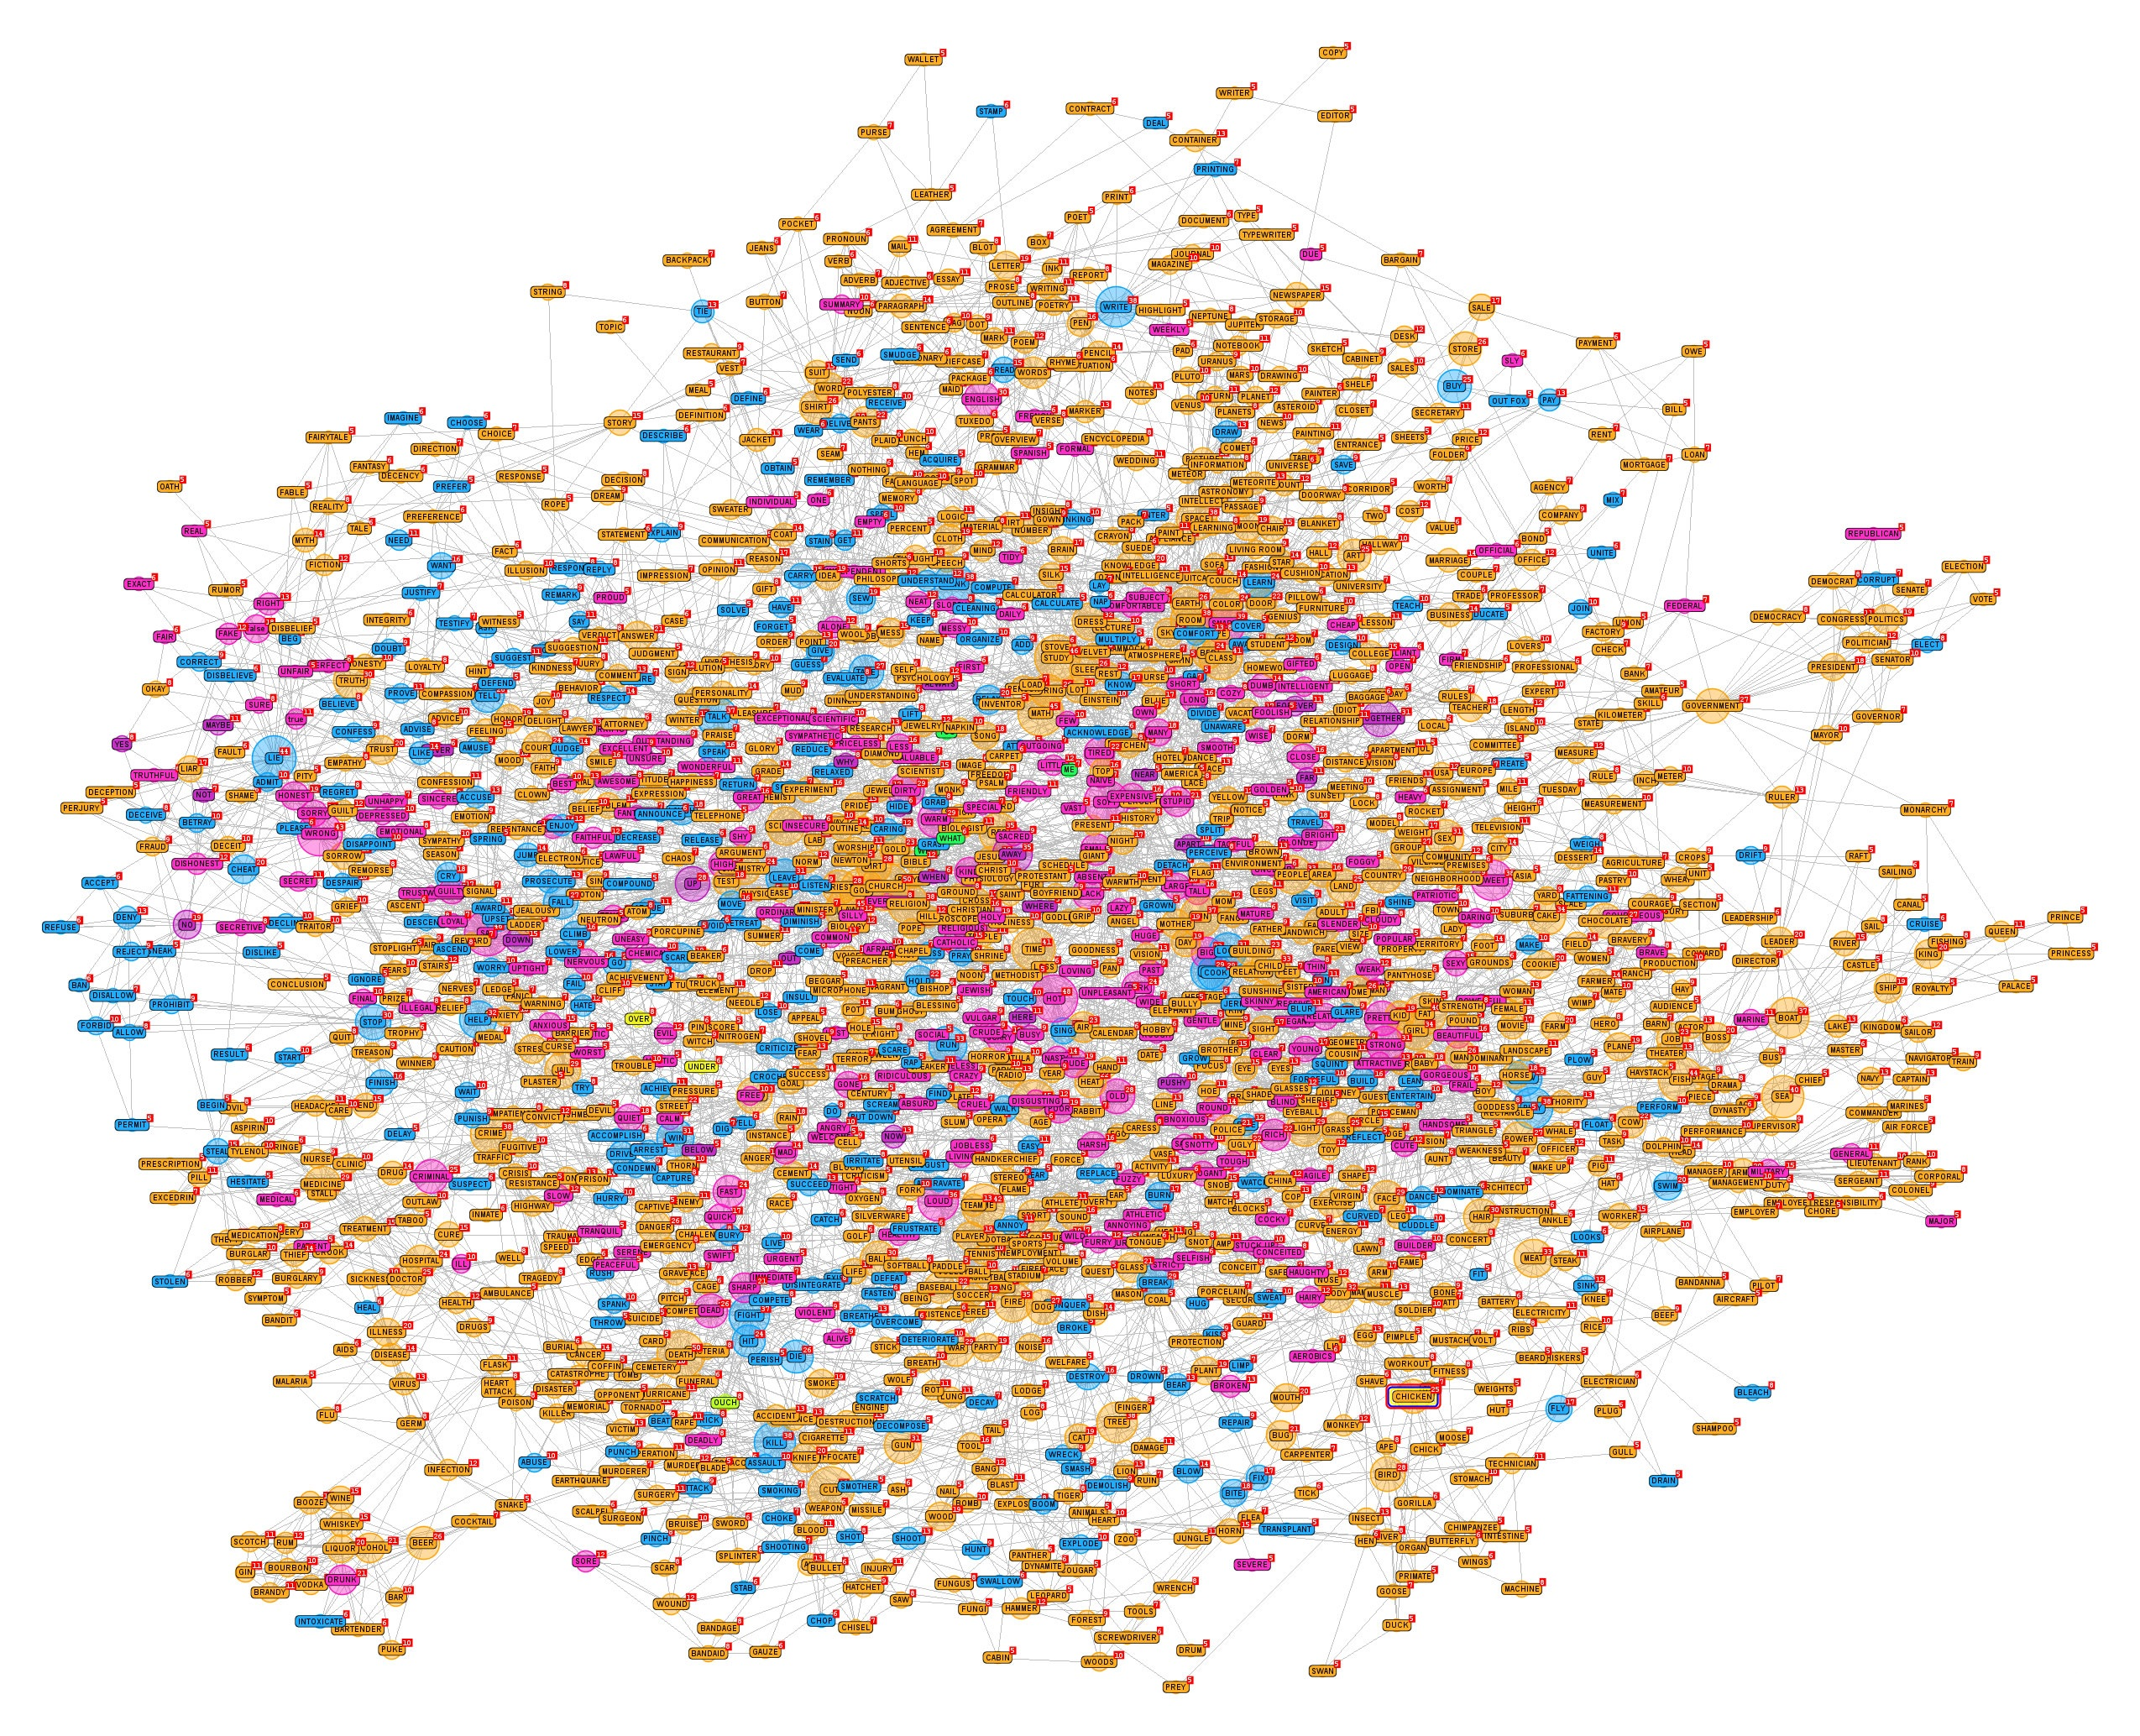
\includegraphics[width=5.0cm,height=5.0cm]{wordassociation.jpg} 
A word association graph using the based on the WordNet database. 

\section{Introduction}
This document is primarily meant to server as a brief tutorial to Natural Language Processing (NLP) as it applies to the problems of classification and prediction of text.  The statistical part comes from the use of corpora and probabilistic models in prediction and classification.  Computational linguistics is an interdisciplinary field dealing with the statistical and/or rule-based modeling of natural language from a computational perspective.  Computational linguistics is primarily concerned with developing algorithms and software for intelligently processing language data and is typically views as a subset of AI.  For our purposes we refer to classification as the process of estimating a categorical variable and prediction as the process of estimating a continuous variable.  For example , assigning a probability for the next word in a string of words is classification, while assigning a vulgarity index to a string of words is regarded as prediction.  A canonical open problem in Computational Linguistics is the automatic translation of one language into another, a task which requires understanding the morphological and syntactical structure of both languages. Other problems in this field include :
\begin{center}
\begin{itemize}
  \item Computational complexity of natural language
  \item Computational semantics
  \item Computer-aided corpus linguistics
  \item Development of parsers for natural languages
  \item Development of taggers to identify parts of speech
  \item Word Sense Disambiguation
\end{itemize}
\end{center}
Some specific problems this document is concerned with are:
\begin{itemize}
  \item Word Completion.  Given a sequence of letters, find the word that best completes the sequence.
  \item Word Prediction. Given a sequence of words, find the word that best completes the sequence.
  \item Document \& Text Classification.
\end{itemize}

While we are primarily interested in a statistical approach to natural language processing, a basic to understanding of syntax and semantics is required to handle the many 'outlier' cases one will encounter.  Modern English has many exceptional rules that must be dealt with.  This document contains two appendices with definitions that reader will want to be familiar with.  Two important tasks in NLP are the decoding of syntactic and semantic information.  These are discussed broadly below.

\subsection{Semantics}
Linguistic semantics refers to the meanings that language elements express.  It typically focuses on the relation between signifiers, such as words, phrases, signs and symbols, and what they stand for.  The term is used in ordinary language to denote a problem of understanding that comes down to word selection or connotation. In written language, such things as paragraph structure and punctuation have semantic content.  The basic unit of semantics is sense.  One word may have many different meanings.  Deriving the meaning from a context - called word sense disambiguation - is a key task in computational linguistics.

\subsection{Lexicography}Lexicography is divided into two related disciplines, practical and theoretical.  Practical lexicography is the art or craft of compiling, writing and editing dictionaries.  Theoretical lexicography is the scholarly discipline of analyzing and describing the semantic, syntagmatic and paradigmatic relationships within the lexicon (vocabulary) of a language, developing theories of dictionary components and structures linking the data in dictionaries, the needs for information by users in specific types of situation, and how users may best access the data incorporated in printed and electronic dictionaries.

\subsection{Corpus linguistics} Corpus linguistics is the study of language as expressed in samples (corpora) or "real world" text. This method represents a digestive approach to deriving a set of abstract rules by which a natural language is governed or else relates to another language. Originally done by hand, corpora are now largely derived by an automated process.


\section{A Quantification the Semantic Information in WordNet}
 WordNet \cite{WORDNET} is a lexical database for the English language. It groups English words into sets of synonyms called synsets, provides short, general definitions, and records the various semantic relations between these synonym sets.  We are interested analyze the statistics of the WordNet semantic graph with the aim to inject sematic information into statistical models.  A "semantic sweetenting" of sorts.

\section{N-gram Models}
N-grams are an important part of NLP tasks like tagging parts of speech, natural language generation [chatterbot engines], plagiarism identification, and character prediction in cell phone text input.  To get an idea of how an  n-gram model is built we will use example n-grams extracted from Anna Kerannina [AK].  The phrase \emph{"for the first time"}, a 4-gram, appears 27 times the body of the novel:
\begin{tiny}
\begin{itemize}
\item saw \emph{for the first} time that inner life of an old, noble,
\item and to make her an offer.  And only then \emph{for the first time} the
\item In Moscow he had \emph{for the first time} felt, after his luxurious and
\item \emph{for the first time} did Vronsky realize clearly the fact that
\item seeing her \emph{for the first time} with all her defects.
\item him \emph{for the first time}.  She was conscious herself that her
\item \emph{For the first time} the question presented itself to him of the
\item feeling.  \emph{For the first time} he pictured vividly to himself her
\item Levin put on his big boots, and, \emph{for the first time}, a cloth
\item And \emph{for the first time} the idea clearly presented itself that it
\item he was going.  He felt utterly wretched.  \emph{For the first time} in
\item mowing this summer \emph{for the first time}.
\item of the men who led this life; but today \emph{for the first time},
\item eagerness, recollecting her son's existence \emph{for the first time}
\item his nose, and \emph{for the first time} in his life he felt on the point
\item death.  Death, the inevitable end of all, \emph{for the first time}
\item moment.  And \emph{for the first time}, for an instant, she felt for
\item with him or separately, that \emph{for the first time} he clearly
\item Now \emph{for the first time} he heard her words with pleasure, and did
\item Vronsky \emph{for the first time} experienced a feeling of anger against
\item Vassenka Veslovsky, obviously \emph{for the first time} in his life
\item "And here we've met \emph{for the first time} since we met at your
\item Jew, or that \emph{for the first time} in his life he was not following
\item talk which he was hearing \emph{for the first time}.  The complexity of
\item it."  And now \emph{for the first time} Anna turned that glaring light
\item for a muslin garment, and going \emph{for the first time} into the frost
\item Then, \emph{for the first time}, grasping that for every man, and
\end{itemize}
\end{tiny}
There are 14200 unique words in the text and 368588 words total.  The frequencies of the unigrams are
{for 2636, the 16579, first 348, time 564}
The unigram \emph{for} appears 2636 times.
The bigram \emph{for the} appears 433 times.
The trigram \emph{for the first} appears 48 times.

We'll come back to these numbers in a moment. Frequencies of the n-grams are presented along with the text in the sequel.

First we need to discuss a subtlety in predicting text.  The two strings \emph{for the} and \emph{for the } are very different when it comes to predicting what comes next.  The bigrams that match the latter in our example text are
\emph{{for the 433, for them 36, for their 21,for these 6,for themselves 6,for they 3, for theirs 1}}
Where there is only one possible bigram matching the former string. Intra word  prediction requires unigram frequencies. The possible matches for continuing \emph{the} are {the 16576, they 998, there 965,them 841,their 689,then 410} We use these counts to define conditional probabilities of the form:
\begin{eqnarray*}
P("the" | "the ") =1 \\
P("the" | "the") = 16579/(16579+998+841+689+401) \\
P("they" | "the" = 998/(16579+998+841+689+401)
\end{eqnarray*}
We refer to the conditional $g$ in $P(w|g)$ as the context, $ g= (w_{1}, ...,w_{i},...,w_{n})$  Using the chain rule this is broken into a product of conditional probabilities,

\begin{eqnarray*}
P(w_{1}, ...,w_{i},...,w_{n}) = P(w_{n}|w_{1} ...,w_{i},...,w_{n-1}) * P(w_{1}, ...,w_{i},...,w_{n-1}) \\
 = P(w_{n}|w_{1} ...,w_{i},...,w_{n-1}) * P(w_{n-1}|w_{1} ...,w_{i},...,w_{n-2}) * P(w_{1}, ...,w_{i},...,w_{n-2})\\
\ldots \\
= P(w_{1}) * P(w_{2} | w_{1}) * P(w_{3} | w_{1} w_{2}) ... P(w_{n} | w_{2} ...w_{n-1})
\end{eqnarray*}
The conditional probabilities are computed using n-grams;
\begin{itemize}
\item unigram $P(w_{i} | g) = P(w_{i})$ \\
\item bigram  $P(w_{i} | g) = P(w_{i} | w_{i-1})$ \\
\item trigram $P(w_{i} | g) =  P(w_{i} | w_{i-1} w_{i-2})$
\end{itemize}
and so forth.  Estimates are obtained from n-gram frequency counts in a training corpus.
to compute the unigram conditional probabilities, $P(w) =  \frac{card(w) }{N}$ Where $N$ is the total number of tokens in the corpus. Bigram conditionals are computed likewise, except that we normalize by the total number of bigrams with the first word $P(w_{i} | w_{i-1}) =  \frac{card( (w_{i-1},w_{i}) ) }{\sum\limits_{w_{n} \in B} card( (w_{i-1},w_{n}))}$

We can calculate the conditionals with our test corpus.  We use $*$ as a wild card.

\[P(for, the, first, time) = P(for)  P(the | for)  P(first | for, the)  P(time | for, the, first)\]

\[P(for, the, first, time) =  \frac{the=16576}{words-368588}  \frac{for, the =433}{for, * = 2663} \frac{for, the, first =48}{for, the * = 433}  \frac{for, the, first, time  =31}{for, the, first, * = 48} \]

\[P(for, the, first, time) =  0.0005235149\]


$P(for the first time)$ as calculated above is bigger than the ratio of \emph{for the first time} to all quad-grams $31/342132 = .0000906083$


\section{Appendix : Syntax}
Syntax is the rule set for constructing sentences in natural languages.  The word is the smallest unit of syntactical structure and a related to each other through rules of grammar.  Traditionally, grammar and syntax dictate that every sentence has a subject and predicate that form the nuclear part of a sentence  The parts of a sentence decorating subject and predicate are termed extranuclear.
There are eight traditional parts of speech (POS) in the English language:
\begin{itemize}
  \item Verb : action or state \emph{Buddha \textbf{climbed} the wall.}
  \item Noun : thing or person \emph{jade}
  \item Adjective : describes a noun \emph{Nice jade Buddha}
  \item Adverb : describes a verb, adjective or adverb \emph{Buddha climbed slowly}
  \item Pronoun : replaces a noun
  \item Preposition : links a noun to another word
  \item Conjunction : joins clauses or sentences or words
  \item Interjection : short exclamation, sometimes inserted into a sentence
\end{itemize}

A more comprehensive POS list used in tagging, stemming, and inflecting text is presented below.
This is from the well known PENN database.  The Penn Treebank Project annotates naturally-occuring text for linguistic structure \cite{PENNTREEBANK}.
\begin{tiny}
\begin{tabular}{|c|c|}
  \hline
Coordinating conjunction	&	CC	\\
Cardinal number	&	CD	\\
Determiner	&	DT	\\
Existential there 	&	EX	\\
Foreign word	&	FW	\\
Preposition or subordinating conjunction	&	IN	 \\
Adjective	&	JJ	\\
Adjective, comparative	&	JJR	\\
Adjective, superlative	&	JJS	\\
List item marker	&	LS	\\
Modal	&	MD	\\
Noun, singular or mass	&	NN	\\
Noun, plural	&	NNS	\\
Proper noun, singular	&	NNP	\\
Proper noun, plural	&	NNPS	\\
Predeterminer	&	PDT	\\
Possessive ending	&	POS	\\
Personal pronoun	&	PRP	\\
Possessive pronoun	&	PRP\$	\\
Adverb	&	RB	\\
Adverb, comparative	&	RBR	\\
Adverb, superlative	&	RBS	\\
Particle	&	RP	\\
Symbol	&	SYM	\\
to	&	TO	\\
Interjection	&	UH	\\
Verb, base form	&	VB	\\
Verb, past tense	&	VBD	\\
Verb, gerund or present participle	&	VBG	\\
Verb, past participle	&	VBN	\\
Verb, non-3rd person singular present	&	VBP	\\
Verb, 3rd person singular present	&	VBZ	\\
Wh-determiner	&	WDT	\\
Wh-pronoun	&	WP	\\
Possessive wh-pronoun	&	WP\$	\\
Wh-adverb	&	WRB	\\
  \hline
\end{tabular}
\end{tiny}

One will generally encounter rule-sets to transform between parts of speech in stemming and inflection engines.


\begin{small}
\subsection{Grammatical Syntactic Definitions}
\subsubsection{adjective}
An adjective is a word whose main syntactic role is to modify a noun or pronoun, giving more information about the noun or pronoun's referent. The adjective order in English is:
\begin{center}
\begin{itemize}
  \item article or pronouns used as adjectives
  \item quality
  \item size
  \item age
  \item shape
  \item color
  \item proper adjective (often nationality or other place of origin)
  \item purpose or qualifier
\end{itemize}
\end{center}
One of the syntactic rules for English prescribes that adjectives describing size precede adjectives pertaining to age.  Another syntactic rule for adjective is that adjectives describing color come after shape. Thus the phrase \emph{"My poor fat old round *"} is a well formed phrase while \emph{"My old square red *"} is not.

\subsubsection{adjunct}
 Adjuncts are optionally omissible parts of a sentence that do not affect the remainder when removed. The sentence: \emph{I won the bike race in the park while it was raining last Saturday}.  Has adjuncts \emph{in the park}, \emph{ while it was raining}, and \emph{last Saturday}.

\subsubsection{adverb}
An adverb is a modifying part of speech describing verbs, other adverbs, adjectives, and phrases. They are used to describe how, where, when, how often, and why something happens.
Adverbs of manner:  \emph{carefully, correctly, eagerly, easily, fast, loudly, patiently,  quickly, quietly, and well}.

Adverbs of place: \emph{abroad, anywhere, downstairs, here, home, in, nowhere, out, outside, somewhere, there, underground, upstairs}.

Adverbs of purpose : \emph{so, so that, to, in order to, because, since, accidentally, intentionally, purposely}.

Adverbs of frequency: \emph{always, every ,never ,often, rarely ,seldom, sometimes, usually}.

Adverbs of time : \emph{after, already, during, finally, just, last, later, next, now, recently, soon}

Adverbs of manner are usually formed by adding \emph{ly} to adjectives. Softly comes from soft, usually come from usual.  The suffix \emph{wise} and \emph{ways} may be used to derive adverbs from nouns. Some adverbs are formed from nouns or adjectives by appending the prefix \emph{a}. There are a number of other suffixes in English that derive adverbs from other word classes, and there are also many adverbs that are not morphologically indicated at all.  Adverbs in English are inflected in terms of comparison like adjectives. The comparative and superlative forms of some single-syllable adverbs that do not end in \emph{ly} are generated by adding \emph{er} and \emph{es}t . Others, especially those ending \emph{ly}, are periphrastically compared by the use of more or most -- while some accept both forms, e.g. oftener and more often are both correct. Adverbs also take comparisons with as ... as, less, and least.  Not all adverbs are comparable; for example in the sentence \emph{He wore red yesterday} it does not make sense to speak of "\emph{more yesterday}" or "\emph{most yesterday}".

\subsubsection{appositive}Apposition is a grammatical construction in which two elements, normally noun phrases, are placed side by side, with one element serving to define or modify the other. When this device is used, the two elements are said to be in apposition. For example, in the phrase \emph{my friend Alice} the name \emph{Alice} is in apposition to \emph{my friend}.  Apposition is a figure of speech of the scheme type, and often results when the verbs (particularly verbs of being) in supporting clauses are eliminated to produce shorter descriptive phrases. This makes them often function as hyperbatons, or figures of disorder, because they can disrupt the flow of a sentence. For example, in the phrase: \emph{My dog, a Papillon with big ears,...}, it is necessary to pause before the parenthetical modification \emph{Papillon with big ears}.

\subsubsection{article}
An article is a word that combines with a noun to indicate the type of reference being made by the noun. Articles specify the grammatical definiteness of the noun, in some languages extending to volume or numerical scope. English articles are \emph{the, and, a, an}.  The word \emph{some} is used as a functional plural of \emph{a, an}.  Articles are considered a special category of adjectives.
Generally common nouns are expressed as definite or indefinite and singular or plural. Every noun must be accompanied by the article, if any, corresponding to its definiteness, and the lack of an article (considered a zero article) itself specifies a certain definiteness. This is in contrast with optional adjectives and determiners.  The compulsory nature of articles makes them the most frequently use words.

\subsubsection{aspect}
The grammatical aspect  of a verb is a grammatical category that defines the temporal flow, or lack thereof, in a given action, event, or state (in a given situation). Commonly the distinction is in how the speaker views the situation, either as unitary and bounded \emph{I ate} or as on-going and unbounded \emph{I was eating}. The distinction here is not in the situation itself, but in the speaker's portrayal of it. Other common aspectual distinctions include whether the situation is repetitive or habitual \emph{I used to eat} or has continuing relevance \emph{I have eaten}. Any one language will have at most a subset of the attested aspectual distinctions made in the world's languages.  Aspect can be a difficult concept to convey and understand intuitively. Because they both convey some sense of time, aspect is often confused with the closely-related concept of tense. While tense relates the time of a situation to some other time, commonly the time of speaking, aspect conveys other temporal information, such as duration, completion, or frequency, as it relates to the time of action. Thus tense refers to temporally when while aspect refers to temporally how. Aspect can be said to describe the texture of the time in which a situation occurs, such as a single point of time, a continuous range of time, a sequence of discrete points in time, etc, whereas tense indicates its location in time.  The concept of aspect is best illustrated by example. Consider the following sentences: \emph{I eat}, \emph{I am eating}, \emph{I have eaten}, and \emph{I have been eating}. All are to some degree in the present tense, as they describe the present situation, yet each conveys different information or points of view as to how the action pertains to the present. As such, they differ in aspect.

\subsubsection{auxiliary verb}
An auxiliary is a verb functioning to give further semantic or syntactic information about the main or full verb following it.  An auxiliary verb alters the basic form of the main verb to make it have one or more of the following functions: passive voice, progressive aspect, perfect aspect, modality, or dummy.
Every clause has a finite verb which consists of a full verb non-auxiliary and optionally one or more auxiliary verbs.
Examples of finite verbs include \emph{write} (no auxiliary verb), \emph{have written} (one auxiliary verb), and \emph{have been written} (two auxiliary verbs).  The primary auxiliary verbs in English are \emph{to be} and \emph{to have}; other major ones include \emph{shall}, \emph{will}, \emph{may} and \emph{can}.

\subsubsection{case}
The case of a noun or pronoun is a change in form that indicates its grammatical function in a phrase, clause, or sentence.  For example, a noun may play the role of subject \emph{I kicked the ball}, of direct object \emph{John kicked me}, or of possessor \emph{My ball}.  More formally, case has been defined as a system of marking dependent nouns for the type of relationship they bear to their heads.

\subsubsection{clause}
A clause is a pair or group of words that consists of a subject and a predicate, although in some languages and some types of clauses the subject may not appear explicitly as a noun phrase. It may instead be marked on the verb (this is especially common in null subject languages). The most basic kind of sentence consists of a single clause. More complicated sentences may contain multiple clauses, including clauses contained within clauses.  Clauses are often contrasted with phrases. Traditionally, a clause was said to have both a finite verb and its subject, whereas a phrase either contained a finite verb but not its subject (in which case it is a verb phrase) or did not contain a finite verb. Hence, in the sentence "I didn't know that the dog ran through the yard," "that the dog ran through the yard" is a clause, as is the sentence as a whole, while "the yard," "through the yard," "ran through the yard," and "the dog" are all phrases. However, modern linguists do not draw the same distinction, as they accept the idea of a non-finite clause, a clause that is organized around a non-finite verb.

\subsubsection{closed class word}
Closed class is a word class to which no new items can normally be added, and that usually contains a relatively small number of items. Typical closed classes found in many languages are adpositions (prepositions and postpositions), determiners, conjunctions, and pronouns.  Contrastingly, an open class offers possibilities for expansion. Typical open classes such as nouns and verbs can and do get new words often, through the usual means such as compounding, derivation, coining, borrowing, etc.  A closed class may get new items through these same processes, but the change takes much more time. The closed class is normally viewed as part of the core language and is not expected to change. Most readers can undoubtedly think of new nouns or verbs entering their lexicon, but it's very unlikely that they can recall any new prepositions or pronouns appearing in the same fashion

\subsubsection{comparative}The comparative is the form of an adjective or adverb which denotes the degree or grade by which a person, thing, or other entity has a property or quality greater or less in extent than that of another, and is used in this context with a subordinating conjunction, such as than, as...as, etc. If three or more items are being compared, the corresponding superlative needs to be used instead.
\subsubsection{complement}Complement is used with different meanings. The primary meaning is a word, phrase or clause which is necessary in a sentence to complete its meaning. We find complements which function as an argument (i.e. of equal status to subjects and objects) and complements which exist within arguments.  Both complements and modifiers add to the meaning of a sentence. However, a complement is necessary to complete a sentence; a modifier is not. For example, "Put the bread on the table" needs "on the table" to make it complete. In most dialects of English, you cannot merely put something; you need to put it somewhere. In this context, the phrase "on the table" is a complement. By contrast, "The bread on the table is fresh." does not require "on the table" to be complete, so here, the phrase "on the table" is a modifier. A modifier, unlike a complement, is an optional element of a sentence

\subsubsection{compound noun and adjective}
 A compound is a lexeme (less precisely, a word) that consists of more than one stem. Compounding or composition is the word formation that creates compound lexemes (the other word-formation process being derivation). Compounding or Word-compounding refers to the faculty and device of language to form new words by combining or putting together old words. In other words, compound, compounding or word-compounding occurs when a person attaches two or more words together to make them one word. The meanings of the words interrelate in such a way that a new meaning comes out which is very different from the meanings of the words in isolation.

\subsubsection{conjugation}Conjugation is the creation of derived forms of a verb from its principal parts by inflection (regular alteration according to rules of grammar). Conjugation may be affected by person, number, gender, tense, aspect, mood, voice, or other grammatical categories. All the different forms of the same verb constitute a lexeme and the form of the verb that is conventionally used to represent the canonical form of the verb (one as seen in dictionary entries) is a lemma. Inflection of nouns and adjectives is known as declension.  Conjugated forms of a verb are called finite forms. In many languages there are also one or more forms that remain unchanged with all or most of grammatical categories: the non-finite forms, such as the infinitive or the gerund. A table giving all the conjugated variants of a verb in a given language is called a conjugation table or a verb paradigm.  Although conjugation tables are a useful tool for the beginner in a foreign language, they fail in irregular verbs. This limitation is particularly prominent in Latin-derived languages like French and Italian. The availability of high power computers has made possible to replace the conjugation tables with conjugation algorithms, that can handle without difficulty the conjugation and the grammar analysis of any verb. However, these are much less useful in understanding the structure of the conjugation forms of a given language.  A regular verb has a set of conventions for conjugation (paradigm) that derives all forms from a few specific forms or principal parts (maybe only one, such as the infinitive in English), in spelling or pronunciation. A verb that has conjugations deviating from this convention is said to be an irregular verb. Typically the principal parts are the root and/or several modifications of it (stems).  Conjugation is also the traditional name of a group of verbs that share a similar conjugation pattern in a particular language (a verb class). This is the sense in which teachers say that Latin has four conjugations of verbs. This means that any regular Latin verb can be conjugated in any person, number, tense, mood, and voice by knowing which of the four conjugation groups it belongs to, and its principal parts

\subsubsection{conjunction}
A conjunction  is a part of speech that connects two words, phrases or clauses together. This definition may overlap with that of other parts of speech, so what constitutes a "conjunction" should be defined for each language. In general, a conjunction is an invariable grammatical particle, and it may or may not stand between the items it conjoins.

The definition can also be extended to idiomatic phrases that behave as a unit with the same function as a single-word conjunction (as well as, provided that, etc.).
1 Coordinating conjunctions
2 Correlative conjunctions
3 Subordinating conjunctions

Coordinating conjunctions, also called coordinators, are conjunctions that join two or more items of equal syntactic importance, such as words, main clauses, or sentences. In English the mnemonic acronym FANBOYS can be used to remember the coordinators \emph{for, and, nor, but, or, yet}, and \emph{so}. These are not the only coordinating conjunctions; various others are used, including \emph{and nor} (British), \emph{but nor} (British), \emph{or nor}(British), \emph{neither} as in \emph{They don't gamble; neither do they smoke}

\emph{for}: presents a reason \emph{He lost all his money, for he gambled too long}
\emph{and}: presents non-contrasting item(s) or idea(s)\emph{ They gamble, and they smoke.}
\emph{or}: presents an alternate item or idea \emph{Every day they gamble or they smoke.}
\emph{nor}: presents a non-contrasting negative idea \emph{They don't gamble, nor do they smoke.}
\emph{but}: presents a contrast or exception \emph{They gamble, but they don't smoke.}
\emph{yet}: presents a contrast or exception \emph{They gamble, yet they don't smoke.}
\emph{so}: presents a consequence \emph{He gambled too long, so he lost all his money.}
Correlative conjunctions are pairs of conjunctions that work together to coordinate two items. English examples include both and, [n]either [n]or, and not [only] but [also], whether... or.

Examples:
\emph{
Either do your work or prepare for a trip to the office.
Not only is he handsome but he is also brilliant.
Neither the basketball team nor the football team is doing well.
Both the cross country team and the swimming team are doing well.
}
\subsubsection{dangling modifier}
A dangling modifier, a specific case of which is the dangling participle, is an error in sentence structure whereby a grammatical modifier is associated with a word other than the one intended, or with no particular word at all. For example, a writer may have meant to modify the subject, but word order makes the modifier seem to modify an object instead. Such ambiguities can lead to unintentional humor or difficulty in understanding a sentence.  A typical example of a dangling modifier is illustrated in the sentence \emph{Turning the corner, a handsome school building appeared}. The modifying clause \emph{Turning the corner} is clearly supposed to describe the behavior of the narrator (or other observer), but grammatically it appears to apply to nothing in particular, or to the school building. Similarly, in the sentence \emph{At the age of eight, my family finally bought a dog}, the modifier \emph{At the age of eight} "dangles" in mid-air, attaching to no named person or thing.

\subsubsection{declension}
Declension is the inflection of nouns, pronouns, adjectives, and articles to indicate number (at least singular vs. plural), case (nominative or subjective, genitive or possessive, etc.), and gender.

\subsubsection{determiner}
A determiner is a noun-modifier that expresses the reference of a noun or noun-phrase in the context, rather than attributes expressed by adjectives. This function is usually performed by articles, demonstratives, possessive determiners, or quantifiers.
\emph{The} girl is \emph{a} student.
I've lost \emph{my} keys.
\emph{Some} folks get \emph{all} the luck.
\emph{Which} book is that?
I only had \emph{two} drinks.
I'll take \emph{that} one.
\emph{Both} windows were open.

\subsubsection{dual }
Dual is a grammatical number that some languages use in addition to singular and plural. When a noun or pronoun appears in dual form, it is interpreted as referring to precisely two of the entities (objects or persons) identified by the noun or pronoun. Verbs can also have dual agreement forms in these languages.
\subsubsection{expletive}
The word expletive is currently used in three senses: syntactic expletives, expletive attributives, and "bad language". Expletive is a term for a meaningless word filling a syntactic vacancy (syntactic expletives).  Sometimes an explicative refers to meaningless, filler, or bad language (expletive attributives), distinguishing this from meaningful use.

\subsubsection{Function word}
Function words (grammatical words or autosemantic words) are words that have little lexical meaning or have ambiguous meaning, but instead serve to express grammatical relationships with other words within a sentence, or specify the attitude or mood of the speaker. Words that are not function words are called content words (or open class words or lexical words): these include nouns, verbs, adjectives, and most adverbs, although some adverbs are function words (e.g., then and why). Dictionaries define the specific meanings of content words, but can only describe the general usages of function words. By contrast, grammars describe the use of function words in detail, but treat lexical words in general terms only.

Function words might be prepositions, pronouns, auxiliary verbs, conjunctions, grammatical articles or particles, all of which belong to the group of closed-class words. Interjections are sometimes considered function words but they belong to the group of open-class words. Function words might or might not be inflected or might have affixes.  Function words belong to the closed class of words in grammar in that it is very uncommon to have new function words created in the course of speech, whereas in the open class of words (that is, nouns, verbs, adjectives, or adverbs) new words may be added readily (such as slang words, technical terms, and adoptions and adaptations of foreign words). See neologism.  Each function word either gives some grammatical information on other words in a sentence or clause, and cannot be isolated from other words, or it may indicate the speaker's mental model as to what is being said.  Grammatical words, as a class, can have distinct phonological properties from content words. Grammatical words sometimes do not make full use of all the sounds in a language.  The following is a list of the kind of words considered to be function words:
\begin{itemize}
    \item articles : the and a.
    \item pronouns : inflected in English, as he - him, she - her, etc.
    \item adpositions : uninflected
    \item conjunctions : uninflected
    \item auxiliary verbs : forming part of the conjugation and are always inflected
    \item interjections  : uninflected
    \item particles : convey the attitude of the speaker and are uninflected, as if, then, well, however, thus, etc.
    \item expletives : take the place of sentences, among other functions.
    \item pro-sentences : yes, okay, etc.
\end{itemize}

\subsubsection{gender}
 Grammatical genders are classes of nouns reflected in the behavior of associated words; every noun must belong to one of the classes and there should be very few that belong to several classes at once.  Modern English is normally described as lacking grammatical gender.

\subsubsection{infinitive}
An infinitive is the name for certain verb forms that exist in many languages. In the usual (traditional) description of English, the infinitive of a verb is its basic form with or without the particle to: therefore, do and to do, be and to be, and so on are infinitives.  In most uses, infinitives are non-finite verbs.  They function as other lexical categories - usually nouns - within the clauses that contain them, for example by serving as the subject of another verb.  They do not represent any of the verb's arguments (as employer and employee do).  They are not inflected to agree with any subject.  They cannot serve as the only verb of a declarative sentence.  They do not have tense, aspect, moods, and/or voice, or they are limited in the range of tenses, aspects, moods, and/or voices that they can use. They are used with auxiliary verbs.

\subsubsection{modal particle}Modal particles are always uninflected words, and are a type of grammatical particle. Their function is that of reflecting the mood or attitude of the speaker or narrator, in that they are not reflexive but change the mood of the verb.

\subsubsection{modifier}
In grammar, a modifier (or qualifier) is an optional element in phrase structure or clause structure; the removal of the modifier typically doesn't affect the grammaticality of the construction. Modifiers can be a word, a phrase or an entire clause. Semantically, modifiers describe and provide more accurate definitional meaning for another element.  In English, adverbs and adjectives prototypically function as modifiers, but they also have other functions. Moreover, other constituents can function as modifiers as the following examples show:
//bbcrevisit this need reworking
adverb in verb phrase: \emph{Put it \textbf{quietly} in the box.}
adverb in adverb phrase : \emph{He put in down \textbf{very quietly}}.
adverb in adjective phrase :\emph{He was very \textbf{gentle}.}
adverb in determiner phrase :\emph{\textbf{Even more} people were there.}
adverb in prepositional phrase \emph{It ran \textbf{right up the tree}.}.
adjective in noun phrase : \emph{It was \textbf{a nice house}.}
noun in noun phrase: \emph{His desk was in \textbf{the faculty office}.}
verb phrase in noun: \emph{\textbf{The swiftly flowing waters} carried it away.}
clause in noun phrase: \emph{I saw the man whom we met yesterday]}.
clause in noun phrase)She's [the woman with the hat].
preposition phrase in noun phrase)It's not [that important]. determiner in adjective phrase) [A few more] workers are needed.
 determiner in determiner phrase)We've already [gone twelve miles]. noun phase in verb phrase
)She's [two inches taller than I].noun phrase in verb adjective phrase)

A premodifier is a modifier placed before the head (the modified component). A postmodifier is a modifier placed after the head, for example:
land mines (pre-modifier)
mines in wartime (post-modifier)
\subsubsection{mood}
Grammatical mood (also mode) is one of a set of morphologically distinctive forms that are used to signal modality.  It is distinct from grammatical tense or grammatical aspect, although these concepts are conflated to some degree in many languages, including English and most other modern Indo-European languages, insofar as the same word patterns are used to express more than one of these concepts at the same time (see Tense-aspect-mood).

Currently identified moods include conditional, imperative, indicative, injunctive, optative, potential, subjunctive, and more. Infinitive is a category apart from all these finite forms, and so are gerunds and participles.

\subsubsection{noun}
A noun is a member of a large, open lexical category whose members can occur as the main word in the subject of a clause, the object of a verb, or the object of a preposition.  A proper noun or proper name is a noun representing unique entities (such as London, Jupiter, or Toyota), as distinguished from common nouns which describe a class of entities (such as city, planet, person or car).  Count nouns are common nouns that can take a plural, can combine with numerals or quantifiers (e.g., one, two, several, every, most), and can take an indefinite article (a or an). Examples of count nouns are chair, nose, and occasion.
Mass nouns (or non-count nouns) differ from count nouns in precisely that respect: they can't take plural or combine with number words or quantifiers. Examples from English include laughter, cutlery, helium, and furniture. For example, it is not possible to refer to a furniture or three furnitures. This is true even though the pieces of furniture comprising furniture could be counted. Thus the distinction between mass and count nouns should not be made in terms of what sorts of things the nouns refer to, but rather in terms of how the nouns present these entities.  Collective nouns are nouns that refer to groups consisting of more than one individual or entity, even when they are inflected for the singular. Examples include committee, herd, and school (of fish). These nouns have slightly different grammatical properties than other nouns. For example, the noun phrases that they head can serve as the subject of a collective predicate, even when they are inflected for the singular.  Concrete nouns refer to physical entities that can, in principle at least, be observed by at least one of the senses (for instance, chair, apple, Janet or atom). Abstract nouns, on the other hand, refer to abstract objects; that is, ideas or concepts (such as justice or hatred). While this distinction is sometimes exclusive, some nouns have multiple senses, including both concrete and abstract ones; consider, for example, the noun art, which usually refers to a concept (e.g., Art is an important element of human culture) but which can refer to a specific artwork in certain contexts (e.g., I put my daughter's art up on the fridge).

Some abstract nouns developed etymologically by figurative extension from literal roots. These include drawback, fraction, holdout, and uptake. Similarly, some nouns have both abstract and concrete senses, with the latter having developed by figurative extension from the former. These include view, filter, structure, and key.  In English, many abstract nouns are formed by adding noun-forming suffixes (-ness, -ity, -tion) to adjectives or verbs. Examples are happiness (from the adjective happy), circulation (from the verb circulate) and serenity (from the adjective serene).

Nouns and noun phrases can typically be replaced by pronouns, such as he, it, which, and those, in order to avoid repetition or explicit identification, or for other reasons. For example, in the sentence \emph{Janet thought that he was weird}, the word \emph{he} is a pronoun standing in place of the name of the person in question. The English word one can replace parts of noun phrases, and it sometimes stands in for a noun. \emph{John's car is newer than the one that Bill has.}  But one can also stand in for bigger subparts of a noun phrase. For example, in the following example, \emph{one} can stand in for new car.  \emph{This new car is cheaper than that one.}


\begin{itemize}
  \item number
  \item object
  \item open class word
  \item part of speech
  \item particle
  \item person
  \item phrase
  \item phrasal verb
  \item plural
  \item predicate (also verb phrase)
  \item predicative (adjectival or nominal)
  \item preposition
  \item personal pronoun
  \item pronoun
  \item Restrictiveness
  \item sentence (linguistics)
  \item singular
  \item subject
  \item superlative
  \item tense
  \item uninflected word
  \item verb
  \item voice
  \item wh-movement
  \item word order
  \item
  \item
\end{itemize}
\end{small}

\subsection{Grammar}
A formal grammar (sometimes simply called a grammar) is a set of rules of a specific kind, for forming strings in a formal language. The rules describe how to form strings from the language's alphabet that are valid according to the language's syntax. A grammar does not describe the meaning of the strings or what can be done with them in whatever context,only their form.
Formal language theory, the discipline which studies formal grammars and languages, is a branch of applied mathematics. Its applications are found in theoretical computer science, theoretical linguistics, formal semantics, mathematical logic, and other areas.
A formal grammar is a set of rules for rewriting strings, along with a "start symbol" from which rewriting must start. Therefore, a grammar is usually thought of as a language generator. However, it can also sometimes be used as the basis for a "recognizer"-a function in computing that determines whether a given string belongs to the language or is grammatically incorrect. To describe such recognizers, formal language theory uses separate formalisms, known as automata theory. One of the interesting results of automata theory is that it is not possible to design a recognizer for certain formal languages.

\subsection{Parsing}
Parsing is the process of recognizing an utterance (a string in natural languages) by breaking it down to a set of symbols and analyzing each one against the grammar of the language. Most languages have the meanings of their utterances structured according to their syntax-a practice known as compositional semantics. As a result, the first step to describing the meaning of an utterance in language is to break it down part by part and look at its analyzed form (known as its parse tree in computer science, and as its deep structure in generative grammar).

\subsection{Generative Grammar}
The hypothesis of generative grammar is that language is a structure of the human mind. The goal of generative grammar is to make a complete model of this inner language (known as i-language). This model could be used to describe all human language and to predict the grammaticality of any given utterance (that is, to predict whether the utterance would sound correct to native speakers of the language). This approach to language was pioneered by Noam Chomsky. Most generative theories (although not all of them) assume that syntax is based upon the constituent structure of sentences. Generative grammars are among the theories that focus primarily on the form of a sentence, rather than its communicative function.

Among the many generative theories of linguistics, the Chomskyan theories are:
\begin{itemize}
  \item Transformational Grammar (TG) (Original theory of generative syntax laid out by Chomsky in Syntactic Structures in 1957)
  \item Government and binding theory (GB) (revised theory in the tradition of TG developed mainly by Chomsky in the 1970s and 1980's).
  \item Minimalist program (MP) (a reworking of the theory out of the GB framework published by Chomsky in 1995)
\end{itemize}



\subsection{Collocation} Within the area of corpus linguistics, collocation defines a sequence of words or terms that co-occur more often than would be expected by chance. The term is often used in the same sense as linguistic government.

Collocation defines restrictions on how words can be used together, for example, which prepositions are used with ("governed by") particular verbs, or which verbs and nouns are typically used together. An example of this (from Michael Halliday) is the collocation strong tea. While the same meaning could be conveyed through the roughly equivalent powerful tea, the fact is that tea is thought of being strong rather than powerful. A similar observation holds for powerful computers, which is preferred over strong computers.

Collocations are examples of lexical units. Collocations should not be confused with idioms although both are similar in that there is a degree of meaning present in the collocation or idiom that is not entirely compositional. With idioms, the meaning is completely non-compositional whereas collocations are mostly compositional.

Collocation extraction is a task that extracts collocations automatically from a corpus, using computational linguistics.

\subsection{Semantic prosody} Semantic prosody, also discourse prosody, describes the way in which certain seemingly neutral words can be perceived with positive or negative associations through frequent occurrences with particular collocations.

An example given by John Sinclair is the combination, set in, which has a negative prosody: rot is a prime example for what is going to set in. Other well-known examples are cause, which is also used mostly in a negative context (accident, catastrophe, etc.), though one can also say that something "caused happiness".

In recent years, linguists have found many hidden associations affecting the neutrality of language, through the use of corpus linguistics and concordancing software. The software is used to arrange Key Words in Context from a corpus of several million words of naturally-occurring text. The collocates can then be arranged alphabetically according to first or second word to the right or to the left. Using such a method, Elena Tognini-Bonelli found that the word largely occurred more frequently with negative words or expressions, while broadly appeared more frequently with positive ones. Lexicographers have often failed to allow for semantic prosody when defining a word, although with the recent development and increasing use of computers, the field of corpus linguistics is now being combined with that of lexicography.

Prosody has also been used to analyze discourse structure. Discourse is not a mere concatenation of utterances; talk is organized in sections through relations between discourse segments, topicality, or other ways. Prosody has been found to correlate with these structures of discourse, notably via key (the pitch of a first prominent syllable in an utterance).

\subsection{Root}
The root is the primary lexical unit of a word, which carries the most significant aspects of semantic content and cannot be reduced into smaller constituents. Content words in nearly all languages contain, and may consist only of, root morphemes. However,sometimes the term "root" is also used to describe the word minus its inflectional endings, but with its lexical endings in place. For example, chatters has the inflectional root or lemma chatter, but the lexical root chat. Inflectional roots are often called stems, and a root in the stricter sense may be thought of as a monomorphemic stem.  The traditional definition allows roots to be either free morphemes or bound morphemes. Root morphemes are essential for affixation and compounds.

The root of a word is a unit of meaning (morpheme) and, as such, it is an abstraction, though it can usually be represented in writing as a word would be. For example, it can be said that the root of the English verb form running is run, or the root of the Spanish superlative adjective amplisimo is ampl-, since those words are clearly derived from the root forms by simple suffixes that do not alter the roots in any way. In particular, English has very little inflection, and hence a tendency to have words that are identical to their roots. But more complicated inflection, as well as other processes, can obscure the root; for example, the root of mice is mouse (still a valid word), and the root of interrupt is, arguably, rupt, which is not a word in English and only appears in derivational forms (such as disrupt, corrupt, rupture, etc.). The root rupt is written as if it were a word, but it's not.

\subsection{Stem}
A stem is a part of a word. The term is used with slightly different meanings.
In one usage, a stem is a form to which affixes can be attached. Thus, in this usage, the English word friendships contains the stem friend, to which the derivational suffix -ship is attached to form a new stem friendship, to which the inflectional suffix -s is attached. In a variant of this usage, the root of the word (in the example, friend) is not counted as a stem.
In a slightly different usage, which is adopted in the remainder of this article, a word has a single stem, namely the part of the word that is common to all its inflected variants. Thus, in this usage, all derivational affixes are part of the stem. For example, the stem of friendships is friendship, to which the inflectional suffix -s is attached.
Stems may be roots, e.g. run, or they may be morphologically complex, as in compound words (cf. the compound nouns meat ball or bottle opener) or words with derivational morphemes (cf. the derived verbs black-en or standard-ize). Thus, the stem of the complex English noun photographer is photo -graph - er, but not photo. For another example, the root of the English verb form destabilized is stabil-, a form of stable that does not occur alone; the stem is de-stabil-ize, which includes the derivational affixes de- and -ize, but not the inflectional past tense suffix -(e)d. That is, a stem is that part of a word that inflectional affixes attach to.

\subsection{Morpheme}
A morpheme is the smallest component of word, or other linguistic unit, that has semantic meaning. The term is used as part of the branch of linguistics known as morpheme-based morphology. A morpheme is composed by phoneme(s) (the smallest linguistically distinctive units of sound) in spoken language, and by grapheme(s) (the smallest units of written language) in written language.  The concept of word and morpheme are different, a morpheme may or may not stand alone. One or several morphemes compose a word. A morpheme is free if it can stand alone (ex: "one", "possible"), or bound if it is used exclusively alongside a free morpheme (ex: "im" in impossible). Its actual phonetic representation is the morph, with the different morphs ("in-", "im-") representing the same morpheme being grouped as its allomorphs.
\subsection{Lexeme}
A lexeme  is an abstract unit of morphological analysis in linguistics, that roughly corresponds to a set of forms taken by a single word. For example, in the English language, run, runs, ran and running are forms of the same lexeme, conventionally written as RUN. A related concept is the lemma (or citation form), which is a particular form of a lexeme that is chosen by convention to represent a canonical form of a lexeme. Lemmas are used in dictionaries as the headwords, and other forms of a lexeme are often listed later in the entry if they are not common conjugations of that word.
A lexeme belongs to a particular syntactic category, has a certain meaning (semantic value), and in inflecting languages, has a corresponding inflectional paradigm; that is, a lexeme in many languages will have many different forms. For example, the lexeme RUN has a present third person singular form runs, a present non-third-person singular form run (which also functions as the past participle and non-finite form), a past form ran, and a present participle running. (It does not include runner, runners, runnable, etc.) The use of the forms of a lexeme is governed by rules of grammar; in the case of English verbs such as RUN, these include subject-verb agreement and compound tense rules, which determine which form of a verb can be used in a given sentence.

\subsection{Word Structure : affix,prefix, suffix}
An affix is a morpheme that is attached to a word stem to form a new word. Affixes may be derivational, like English \emph{ness} and \emph{pre}, or inflectional, like English plural \emph{s} and past tense \emph{ed}. They are bound morphemes by definition; prefixes and suffixes may be separable affixes. Affixation is, thus, the linguistic process speakers use to form new words (neologisms) by adding morphemes (affixes) at the beginning (prefixation), the middle (infixation) or the end (suffixation) of words.

A prefix is an affix which is placed before the stem of a word. Particularly in the study of Semitic languages, a prefix is called a preformative, because it alters the form of the words to which it is affixed.
\begin{itemize}
  \item unhappy : un is a negative or antonymic prefix.
  \item prefix, preview : pre is a prefix, with the sense of before
  \item redo, review : re is a prefix meaning again
\end{itemize}

A suffix is an affix which is placed after the stem of a word. Examples are case endings, which indicate the grammatical case of nouns or adjectives, and verb endings, which form the conjugation of verbs.
Suffixes can carry grammatical information (inflectional suffixes) or lexical information (derivational suffixes). An inflectional suffix is sometimes called a desinence.
\begin{itemize}
  \item \emph{Girls} where the suffix \emph{s} marks the plural.
  \item \emph{He makes} where suffix \emph{s} marks the third person singular present tense.
  \item \emph{It closed} where the suffix \emph{ed} marks the past tense
\end{itemize}
Inflection changes grammatical properties of a word within its syntactic category.
\emph{The weather forecaster said it would clear today, but it hasn't cleared at all.}
the suffix \emph{ed} inflects the root-word \emph{clear} to indicate past tense.

Inflectional English suffixes:

\emph{s} third person singular present
\emph{ed} past tense
\emph{ing} progressive/continuous
\emph{en} past participle
\emph{s} plural
\emph{en} plural (irregular)
\emph{er} comparative
\emph{est} superlative
\emph{n't} negative

In the sentence \emph{The weather forecaster said it would be clear today, but I can't see clearly at all}
the suffix \emph{ly} modifies the root-word clear from an adjective into an adverb.

Derivation can also form a semantically distinct word within the same syntactic category.  \emph{The weather forecaster said it would be a clear day today, but I think it's more like clearish!}
The suffix \emph{ish} modifies the root-word clear, changing its meaning to "clear, but not very clear".

English derivational suffixes :
\emph{ian}
\emph{ize/ise}
\emph{fy}
\emph{ly}
\emph{ful}
\emph{able/ible}
\emph{hood}
\emph{ness}
\emph{less}
\emph{ism}
\emph{ment}
\emph{ist}
\emph{al}
\emph{ish}

\subsection{Lemma}
In linguistics a lemma (plural lemmas or lemmata) is either of two things:
\begin{itemize}
  \item Morphology, lexicography: the canonical form, dictionary form, or citation form of a set of words (headword); e.g., in English, run, runs, ran and running are forms of the same lexeme, with run as the lemma.
  \item Psycholinguistics: abstract conceptual form that has been mentally selected for utterance in the early stages of speech production, but before any sounds are attached to it.
A lemma in morphology is the canonical form of a lexeme. Lexeme, in this context, refers to the set of all the forms that have the same meaning, and lemma refers to the particular form that is chosen by convention to represent the lexeme. In lexicography, this unit is usually also the citation form or headword by which it is indexed. Lemmas have special significance in highly inflected languages such as Czech. The process of determining the lemma for a given word is called lemmatisation.
\end{itemize}
The psycholinguistics interpretation refers to one of the more widely accepted psycholinguistic models of speech production, referring to an early stage in the mental preparation for an utterance. Here, lemma is the abstract form of a word that arises after the word has been selected mentally, but before any information has been accessed about the sounds in it (and thus before the word can be pronounced). It therefore contains information concerning only meaning and the relation of this word to others in the sentence.

\subsection{Differences Between a Stem and a Lemma}
A stem is the part of the word that never changes even when morphologically inflected, whilst a lemma is the base form of the verb. For example, from "produced", the lemma is "produce", but the stem is "produc-." This is because there are words such as production. In linguistic analysis, the stem is defined more generally as the analyzed base form from which all inflected forms can be formed. When phonology is taken into account, the definition of the unchangeable part of the word is not useful, as can be seen in the phonological forms of the words in the preceding example: "produced", "production".  Some lexemes have several stems but one lemma. For instance "to go" (the lemma) has the stems "go" and "wend". (The past tense is based on a different verb, "to wend". The "-t" suffix may be considered as equivalent to "-ed".)

\subsection{Lexicon}
The lexicon of a language is its vocabulary, including its words and expressions. More formally, it is a language's inventory of lexemes. The lexicon includes the lexemes used to actualize words. Lexemes are formed according to morpho-syntactic rules and express sememes. In this sense, a lexicon organizes the mental vocabulary in a speaker's mind: First, it organizes the vocabulary of a language according to certain principles (for instance, all verbs of motion may be linked in a lexical network) and second, it contains a generative device producing (new) simple and complex words according to certain lexical rules. For example, the suffix \emph{able} can be added to transitive verbs only, so that we get \emph{readable} but not \emph{cryable}.  Usually a lexicon is a container for words belonging to the same language.
\subsection{Morphology}
Morphology is the identification, analysis and description of the structure of morphemes and other units of meaning in a language like words, affixes, and parts of speech and intonation/stress, implied context (words in a lexicon are the subject matter of lexicology). Morphological typology represents a way of classifying languages according to the ways by which morphemes are used in a language from the analytic that use only isolated morphemes, through the agglutinative ("stuck-together") and fusional languages that use bound morphemes (affixes), up to the polysynthetic, which compress lots of separate morphemes into single words.

Words are generally accepted as being the smallest units of syntax,and are related to other words by rules of grammar. For example, English speakers recognize that the words dog and dogs are closely related - differentiated only by the plurality morpheme "-s," which is only found bound to nouns, and is never separate. Speakers of English (a fusional language) recognize these relations from their tacit knowledge of the rules of word formation in English. They infer intuitively that dog is to dogs as cat is to cats; similarly, dog is to dog catcher as dish is to dishwasher (in one sense). The rules understood by the speaker reflect specific patterns (or regularities) in the way words are formed from smaller units and how those smaller units interact in speech. In this way, morphology is the branch of linguistics that studies patterns of word formation within and across languages, and attempts to formulate rules that model the knowledge of the speakers of those languages. A morpheme is the smallest component of word, or other linguistic unit, that has semantic meaning. The term is used as part of the branch of linguistics known as morpheme-based morphology. A morpheme is composed by phoneme(s) (the smallest linguistically distinctive units of sound) in spoken language, and by grapheme(s) (the smallest units of written language) in written language.

The concept of word and morpheme are different, a morpheme may or may not stand alone. One or several morphemes compose a word. A morpheme is free if it can stand alone (ex: "one", "possible"), or bound if it is used exclusively alongside a free morpheme (ex: "im" in impossible). Its actual phonetic representation is the morph, with the different morphs ("in-", "im-") representing the same morpheme being grouped as its allomorphs.   The word "unbreakable" has three morphemes: "un-", a bound morpheme; "break", a free morpheme; and "-able", a free morpheme. "un-" is also a prefix, "-able" is a suffix. Both "un-" and "-able" are affixes.  In morphology, a bound morpheme is a morpheme that cannot stand alone as an independent word. A free morpheme is one which can stand alone.  Most English language affixes (prefixes and suffixes) are bound morphemes, e.g., -ment in "shipment", or pre- in "prefix".  Many roots are free morphemes, e.g., ship- in "shipment", while others are bound. The morpheme ten- in "tenant" may seem free, since there is an English word "ten". However, its lexical meaning is derived from the Latin word tenere, "to hold", and this or related meaning is not among the meanings of the English word "ten", hence ten- is a bound morpheme in the word "tenant".

There are some distinguished types of bound morphemes.  A  unique morpheme is one with extremely limited distribution so that it occurs in only one word. A popular example is cran- in cranberry" (hence the term "cranberry morpheme"), although this example is something of a technicality given that it is an alteration or contraction of the free morpheme "crane".  Unique morphemes are examples of the linguistic notion of fossilization: loss of productivity or usage of grammar units: words, phrases, parts of words. Besides fossilized root morphemes, there are also fossilized affixes (suffixes and prefixes).

\subsection{Inflection}
In grammar, inflection or inflexion is the modification of a word to express different grammatical categories such as tense, mood, voice, aspect, person, number, gender and case. Conjugation is the inflection of verbs; declension is the inflection of nouns, adjectives and pronouns.

Inflection can be overt or covert within the same language. An overt inflection expresses grammatical category with an explicitly stated suffix. In English, the word "lead" is not marked for either person or number, and is only marked for tense in opposition to "led" (i.e. is not specifically future tense). The whole clause, however, achieves all the grammatical categories by the inclusion of extra words. This is covert inflection (or periphrasis).  The process typically distinguishes lexical items (such as lexemes) from functional ones (such as affixes, clitics, particles and morphemes in general) and has functional items acting as markers on lexical ones.

Lexical items that do not respond to overt inflection are invariant or uninflected; for example, "must" is an invariant item: it never takes a suffix or changes form to signify a different grammatical category. Its category can only be determined by its context. Uninflected words do not need to be lemmatized in linguistic descriptions or in language computing. On the other hand, inflectional paradigms, or lists of inflected forms of typical words (such as sing, sang, sung, sings, singing, singer, singers, song, songs, songstress, songstresses in English) need to be analyzed according to criteria for uncovering the underlying lexical stem (here s*ng-); that is, the accompanying functional items (-i-, -a-, -u-, -s, -ing, -er, -o-, -stress, -es) and the functional categories of which they are markers need to be distinguished to adequately describe the language.

Constraining the cross-referencing of inflection in a sentence is known as concord or agreement. For example, in "the choir sings", "choir" and "sings" are constrained to the singular number; if one is singular, they both must be.

Languages that have some degree of overt inflection are inflected languages. The latter can be highly inflected, such as Latin (overtly), or weakly inflected, such as English (covertly), depending on the presence or absence of overt inflection. And, historically, English was traditionally described as a non-inflected Indo-European language.

\subsection{Derivation}
Derivation is  the process by which new words, as with \emph{happiness} and \emph{unhappy} from \emph{happy}, or \emph{determination} from \emph{determine}. A contrast is intended with the process of inflection, which uses another kind of affix in order to form variants of the same word, as with \emph{determine/determine-s/determin-ing/determin-ed}.  A derivational suffix usually applies to words of one syntactic category and changes them into words of another syntactic category. For example, the English derivational suffix \emph{ly} changes adjectives into adverbs

\subsection{Inflection Versus Derivation}
Inflection is the process of adding inflectional morphemes (smallest units of meaning) to a word, which indicate grammatical information (for example, case, number, person, gender or word class, mood, tense, or aspect). Derivation is the process of adding derivational morphemes, which create a new word from existing words, sometimes by simply changing grammatical category (for example, changing a noun to a verb).  Words generally are not listed in dictionaries (in which case they would be lexical items) on the basis of their inflectional morphemes. But they often are listed on the basis of their derivational morphemes. For instance, English dictionaries list readable and readability, words with derivational suffixes, along with their root read. However, no traditional English dictionary lists book as one entry and books as a separate entry nor do they list jump and jumped as two different entries.

\subsection{Inflectional Morphology}
Languages that add inflectional morphemes to words are sometimes called inflectional languages, which is a synonym for inflected languages. Morphemes may be added in several different ways:
\begin{itemize}
  \item Affixation, or simply adding morphemes onto the word without changing the root
\item Reduplication, doubling all or part of a word to change its meaning
\item Alternation, exchanging one sound for another in the root
\end{itemize}
Suprasegmental variations, such as of stress, pitch or tone, where no sounds are added or changed but the intonation and relative strength of each sound is altered regularly. For an example, see Initial-stress-derived noun.

Affixing includes prefixing (adding before the base), and suffixing (adding after the base), as well as the much less common infixing (inside) and circumfixing (a combination of prefix and suffix).Inflection is most typically realized by adding an inflectional morpheme (that is, affixation) to the base form (either the root or a stem).
\subsection{Fossilization}
In linguistic morphology, fossilization refers to two close notions. One is preserving of ancient linguistic features which have lost their grammatical functions in language. Another is loss of productivity of a grammatical paradigm (e.g., of an affix), which still remains in use in some words.
Examples of fossilization include fossilized morphemes and fossil words.  A fossil word is an obsolete word which remains in currency because it is contained within an idiom still in use.  It can also occur for phrases, such as in point ('relevant'), which is retained in the larger phrases case in point and in point of fact, but is not otherwise used outside of a legal context.

\begin{center}
English language examples:
Ulterior, as in 'ulterior motives'
Ilk, as in 'of that ilk'
Fro, as in 'to and fro'
Sleight, as in 'sleight of hand'
Yore, as in 'days of yore'
Coign, as in 'coign of vantage'
Deserts, as in 'just deserts'
Craw, as in 'sticks in one's craw'
Fettle, as in 'in fine fettle'
Kith, as in 'kith and kin'
Spick, as in 'spick and span'
Loggerheads as in 'at loggerheads'
Offing, as in 'in the offing'
Shrift, as in 'short shrift'
Amok, as in 'run amok'
\end{center}

\subsection{Stemming}
Stemming is the process for reducing inflected (or sometimes derived) words to their stem, base or root form - generally a written word form. The stem need not be identical to the morphological root of the word; it is usually sufficient that related words map to the same stem, even if this stem is not in itself a valid root. The algorithm has been a long-standing problem in computer science; the first paper on the subject was published in 1968. The process of stemming, often called conflation, is useful in search engines for query expansion or indexing and other natural language processing problems.  Stemming programs are commonly referred to as stemming algorithms or stemmers.

\subsubsection{Brute Force Stemming}
Brute force stemmers employ a lookup table which contains relations between root forms and inflected forms. To stem a word, the table is queried to find a matching inflection. If a matching inflection is found, the associated root form is returned. Brute force approaches are criticized for their general lack of elegance in that no algorithm is applied that would more quickly converge on a solution. In other words, there are more operations performed during the search than should be necessary. Brute force searches consume immense amounts of storage to host the list of relations (relative to the task). The algorithm is only accurate to the extent that the inflected form already exists in the table. Given the number of words in a given language, like English, it is unrealistic to expect that all word forms can be captured and manually recorded by human action alone. Manual training of the algorithm is overly time-intensive and the ratio between the effort and the increase in accuracy is marginal at best.

\subsubsection{Production Stemming}
Some programs attempt to automatically generate the table of root and inflected forms. A production algorithm attempts to infer the probable inflections for a given word. For example, if the word is "run", then the algorithm might automatically generate the forms "running" and "runs". In the traditional sense of the concept of stemming, this algorithm is its reverse process. Rather than try and remove suffixes, the goal of a production algorithm is to generate suffixes. Later, a brute force algorithm can simply query the automatically generated table of word relations to find the root form of a word.
There are many types of heuristic, experimental techniques for identifying inflected forms of words. Some algorithms work phonetically, looking at the final syllables in a word. Some are rather brute force, using rules that seem a lot like normalization rules, by inspecting the last few characters. Others are similar to the process of lemmatisation, which takes advantage of the additional knowledge about the part of speech of the given word to limit what types of suffixes are considered when generating inflections for the word.

\subsubsection{Suffix Stripping}
Suffix stripping algorithms do not rely on a lookup table that consists of inflected forms and root form relations. Instead, a typically smaller list of "rules" are stored which provide a path for the algorithm, given an input word form, to find its root form. Some examples of the rules include:
"	if the word ends in 'ed', remove the 'ed'
"	if the word ends in 'ing', remove the 'ing'
"	if the word ends in 'ly', remove the 'ly'
Suffix stripping approaches enjoy the benefit of being much simpler to maintain than brute force algorithms, assuming the maintainer is sufficiently knowledgeable in the challenges of linguistics and morphology and encoding suffix stripping rules. Suffix stripping algorithms are sometimes regarded as crude given the poor performance when dealing with exceptional relations (like 'ran' and 'run'). The solutions produced by suffix stripping algorithms are limited to those lexical categories which have well known suffixes with few exceptions. This, however, is a problem, as not all parts of speech have such a well formulated set of rules. Lemmatisation attempts to improve upon this challenge.

\subsubsection{Stochastic Stemming and Lemmatization Algorithms}
Stochastic algorithms involve using probability to identify the root form of a word. Stochastic algorithms are trained (they "learn") on a table of root form to inflected form relations to develop a probabilistic model. This model is typically expressed in the form of complex linguistic rules, similar in nature to those in suffix stripping or lemmatisation. Stemming is performed by inputting an inflected form to the trained model and having the model produce the root form according to its internal ruleset, which again is similar to suffix stripping and lemmatisation, except that the decisions involved in applying the most appropriate rule, or whether or not to stem the word and just return the same word, or whether to apply two different rules sequentially, are applied on the grounds that the output word will have the highest probability of being correct (which is to say, the smallest probability of being incorrect, which is how it is typically measured).
Some lemmatisation algorithms are stochastic in that, given a word which may belong to multiple parts of speech, a probability is assigned to each possible part. This may take into account the surrounding words, called the context, or not. Context-free grammars do not take into account any additional information. In either case, after assigning the probabilities to each possible part of speech, the most likely part of speech is chosen, and from there the appropriate normalization rules are applied to the input word to produce the normalized (root) form.

\subsubsection{Stochastic N-Gram Stemming}
To further explain, consider the well known technique of n-gram analysis. Here the term gram is a unit of measurement of text that may refer to a single character, a single syllable, or a single word. Which one applies is dependent upon which author or programmer is describing the algorithm (and their background, as a linguist is more likely to be referring to syllables, but a computer scientist characters and a software company words). The prefix n is, as usual in computer science jargon, representing 'any number of', or a 'variable number of'. There are frequently used subsets of n-grams, such as bigrams (a.k.a digrams, bi-grams, di-grams), representing a sequence of two grams (two characters or two words or two syllables in a row, consecutively in the text). Trigrams (three units) are also popular.
In language modeling, one could write a software program that stores a large table of all word bigrams found in a large body of text (called a corpus). The algorithm would scan word by word, like a sliding window, across the text from the beginning, storing two word sequences as it moves along until the last word of the last document is reached. On the output, one has what is called a bigrams table. Each row in the table may be called a tuple, storing the first word, and then the second word. Additional characteristics may be stored about each bigram, such as its frequency (the total count of the times the whole bigram was discovered) in whatever body of texts was used to generate the table. The table may also store the frequency of each individual word. For example, this sentence contains bigrams like "for example" and "this sentence".
From the table an algorithm can garner the probability of the second word following the first word by assessing each word's frequency and the frequency of the bigrams and perhaps other criteria like the total number of bigrams or the total number of bigrams where the first word is the same. For example, one would be able to state conclusions like: the presence of the word post indicates a probability of the following word being office of 50\%, because the sequence occurred this way 50\% of the time in the text (where post occurred with and without office following it).  In the bi-gram relationship, the first word can be understood as the context that describes the second word. It qualifies the second word, providing additional insight into its meaning. Humans use the technique of examining the context of words to determine the meaning of written words quite frequently. Words can have multiple meanings, called senses. The bigram-provided context provides a way to distinguish which sense of the word is used (well, most of the time, as literary puns and the like are the obvious exception). As mentioned elsewhere, the stemming algorithm can use this context as additional information to assist in determining the outcome of the algorithm (whether or not the current word is stemmed, which of one or more possible stems is appropriate, whether to use substitution or stripping, whether the word is a verb or noun or some other lexical category, etc). Because the algorithm used probabilities in determining the outcome, it is a stochastic algorithm.
Entering into the realm of stochastic algorithms may greatly complicate the stemming algorithm, making it much harder to develop, distribute and maintain. There is considerable debate over its benefits. If a simple suffix stripper can get to about 80\% accuracy from a few days or weeks of programming, then how much more valuable is it that a context-driven n-gram stemmer can achieve 90\% accuracy given several months of work? There are also many problems with stochastic stemmers. What if the body of text used to derive the probabilities of the bigrams is not a representative sample of all documents ever written in a given language (and it is likely not)? What if the algorithm's bigram table 'becomes corrupted', by learning from 'bad text'? Reconfiguring a brute force algorithm that employs a lookup table is as simple as going in and removing a row from the table. But how does one reconfigure a probabilistic network (this is analogous to some of the problems behind neural networks)?

\section{Appendix : Semantics}
Words can be related by various attributes such as similarity, membership, or by lexical relations through morphological constructs.  Morphological categorization into different grammatical categories such as tense, mood, voice, aspect, person, number, gender and case is generally accomplished through the rules of inflection.  We use WordNet as a source for semantic relationships, and discuss the concepts of semantics within the framework of the WordNet model.

\subsection{Word Relationships in the WordNet database }
 WordNet \cite{WORDNET} is a lexical database for the English language. It groups English words into sets of synonyms called synsets, provides short, general definitions, and records the various semantic relations between these synonym sets.  Synonymy is a lexical relation between word forms. It is assigned a central role in WordNet. Semantic relations are indicated by pointers to other words. WordNet is organized by semantic relations. A semantic relation is a relation between meanings and since meanings can be represented by synsets.  It is natural to think of semantic relations as pointers between synsets. It is characteristic of semantic relations that they are reciprocated: if there is a semantic relation R between meaning {x, x0, . . .} and meaning {y, y0, . . .}, then there is also a relation R~ between {y, y0, . . .} and {x, x0, . . .}.

Semantic Relations Found In WordNet:

\textbf{Nouns}
\begin{itemize}
  \item hypernyms: Y is a hypernym of X if every X is a (kind of) Y (canine is a hypernym of dog, because every dog is a member of the larger category of canines)

  \item hyponyms: Y is a hyponym of X if every Y is a (kind of) X (dog is a hyponym of canine)

  \item coordinate terms: Y is a coordinate term of X if X and Y share a hypernym (wolf is a coordinate term of dog, and dog is a coordinate term of wolf)
   \item   holonym: Y is a holonym of X if X is a part of Y (building is a holonym of window)
    \item meronym: Y is a meronym of X if Y is a part of X (window is a meronym of building)

\end{itemize}


\textbf{Verbs}
\begin{itemize}
\item hypernym: the verb Y is a hypernym of the verb X if the activity X is a (kind of) Y (to perceive is an hypernym of to listen)
\item troponym: the verb Y is a troponym of the verb X if the activity Y is doing X in some manner (to lisp is a troponym of to talk)
\item entailment: the verb Y is entailed by X if by doing X you must be doing Y (to sleep is entailed by to snore)
\item coordinate terms: those verbs sharing a common hypernym (to lisp and to yell)
\end{itemize}

\textbf{Adjectives}
\begin{itemize}
\item elated nouns
\item similar to
\item participle of verb
\item Adverbs
\item root adjectives
\end{itemize}

Nouns are organized from a set of base classes in WordNet - so called 'Primes'
{act, action, activity}
{natural object}
{animal, fauna}
{natural phenomenon}
{artifact}
{person, human being}
{attribute, property}
{plant, flora}
{body, corpus}
{possession}
{cognition, knowledge}
{process}
{communication}
{quantity, amount}
{event, happening}
{relation}
{feeling, emotion}
{shape}
{food}
{state, condition}
{group, collection}
{substance}
{location, place}
{time}
{motive}


\subsubsection{Antonym}
The antonym of a word x is sometimes not-x, but not always. For example, rich
and poor are antonyms, but to say that someone is not rich does not imply that they mustbe poor; many people consider themselves neither rich nor poor. Antonymy, which seems to be a simple symmetric relation, is actually quite complex, yet speakers of English have little difficulty recognizing antonyms when they see them. Antonymy is a lexical relation between word forms, not a semantic relation between word meanings. For example, the meanings {rise, ascend} and {fall, descend} may be conceptual opposites, but they are not antonyms; [rise/fall] are antonyms and so are [ascend/descend], but most people hesitate and look thoughtful when asked if rise and descend, or ascend and fall, are antonyms. Such facts make apparent the need to distinguish between semantic relations between word forms and semantic relations between word meanings. Antonymy provides a central organizing principle for the adjectives and adverbs in WordNet, and the complications that arise from the fact that antonymy is a semantic relation between words are better discussed in that context.
\subsubsection{Hyponym}
hyponymy/hypernymy is a semantic relation between word meanings: e.g., {maple} is a hyponym of {tree}, and {tree} is a hyponym of {plant}. Much attention has been devoted to hyponymy/hypernymy (variously called subordination/superordination, subset/superset, or the \emph{ISA} relation).

\begin{itemize}
\item member holynym
\item substance holonym
\item part holonym
\end{itemize}

%\subsubsection{instance hyponym}


\subsubsection{Meronym}
The part-whole (or HASA) relation, known to lexical semanticists as meronymy/holonymy.   The meronymic relation is transitive (with qualifications) and asymmetrical, and can be used to construct a part hierarchy (with some reservations, since a meronym can have many holonyms).
\begin{itemize}
\item member meronym
\item substance meronym
\item part meonym
\end{itemize}


\subsubsection{Entailment}
In logic, entailment, or strict implication, is properly defined for propositions; a proposition P entails a proposition Q if and only if there is no conceivable state of affairs that could make P true and Q false. Entailment is a semantic relation because it involves reference to the states of affairs that P and Q represent. The term will be generalized here to refer to the relation between two verbs V1 and V2 that holds when the sentence Someone V1 logically entails the sentence Someone V2; this use of entailment can be called lexical entailment. Thus, for example, snore lexically entails sleep because the sentence He is snoring entails He is sleeping; the second sentence necessarily holds if the the first one does. Lexical entailment is a unilateral relation: if a verb V1 entails another verb V2, then it cannot be that case that V2 entails V1. The exception is that where two verbs can be said to be mutually entailing, they must also be synonyms, that is, they must have the same sense. For example, one might say both that The Germans beat the Argentinians entails The Germans defeated the Argentinians, and that The Germans defeated the Argentinians entails The Germans beat the Argentinians. However, we find such statements rather unnatural. Negation reverses the direction of entailment: not sleeping entails not snoring, but not snoring does not entail not sleeping. The converse of entailment is contradiction: If the sentence He is snoring entails He is sleeping, then He is snoring also contradicts the sentence He is not sleeping. The entailment relation between verbs resembles meronymy between nouns, but meronymy is better suited to nouns than to verbs. To begin with, in order for sentences based on the formula An x is a part of a y to be acceptable, both x and y must be nouns. It might seem that using the nominalizing gerundive form of the verbs would convert them into nouns, and as nouns the HASA relation should apply.

\subsubsection{Other WordNet Relation Types}
\begin{itemize}
\item cause
\item also see
\item derived from
\item attribute
\item relational adj
\item similar to
\item verb group
\item participle
\item attribute
\item derivationally related
\item domain topic
\item member topic
\item domain region
\item member region
\item domain usage
\item member usage
\item pertainym
\item same
\item equivalent
\item subsuming
\item instance
\item antiequivalent
\item antisubsuming
\item antiinstance
\end{itemize}


\footnotesize
\begin{thebibliography}{99}

\bibitem{SBAR} http://www.cs.sunysb.edu/~algorith {\em The Stony Brook Algorithm Repository}
\bibitem{NISTDADS} http://xw2k.nist.gov/dads {\em NIST Dictionary of Algorithms and Data Structures}
\bibitem{PENNTREEBANK} http://www.cis.upenn.edu/~treebank/ {\em The Penn Treebank Project}
\bibitem{WORDNET} http://wordnet.princeton.edu/ {\em WordNet - a large lexical database of English}
\bibitem{WIKI} http://www.wikipedia.org/
\end{thebibliography}



